%======================================================================
\section{Track AUT --- AI and automation}\label{sec:aut}
%======================================================================

\begin{epic}{AUT-01}{Headless hooks \& CLI}{M0}{\stDone}{FCB-P2-11..14}
Merged in \#5: \file{addons/BruceWorx/hooks.py} exports STEP, lists the document tree as JSON, and
numbers and renames parts through FreeCADCmd. Every later automation epic builds on it.
\end{epic}

\begin{epic}{AUT-02}{bruceworx.api}{M1}{\stTodo}{FCB-P2AI-03}
A stable Python module over the hooks: create and edit parts, set parameters (\eref{MOD-02}), read the tree,
export STEP/STL/3MF, run inspections (\eref{MOD-11}). One undo transaction per call.
\emph{Acceptance:} the API is covered by headless tests in CI.
\end{epic}

\begin{epic}{AUT-03}{MCP server}{M1}{\stTodo}{FCB-P2AI-01/02, 04..08}
Choose a base among the MIT and LGPL FreeCAD MCP servers (spike plus gate, including whether raw
\code{execute\_code} is allowed), then add BruceWorx tools: tree, create/edit, export, numbering, COTS
insert, mass report. Includes a headless mode on FreeCADCmd for cloud agents, and security: localhost by
default, a token, and an audit log. Configuration docs for the agents in use, and integration tests in CI.
\emph{Acceptance:} an agent creates, queries and exports a part headless in CI.
\end{epic}

\begin{epic}{AUT-04}{Assistant panel}{M5}{\stTodo}{FCB-P2AI-09..15}
A dock with chat, a tool-call preview, and apply/undo per action. It calls \code{bruceworx.api} and MCP, and
gets a UX mock and design gate first.
\emph{Acceptance:} a try-out on real CAD work is signed off.
\end{epic}

\begin{epic}{AUT-05}{Command line}{M5}{\stTodo}{(new, from the UI plan)}
A bottom command line accepting AutoCAD-style aliases, inline Python, CadQuery/build123d scripts and
OpenSCAD, plus a \code{CodeFeature} that keeps a script as a parametric, trust-gated feature.
\emph{Acceptance:} \code{CPATTERN @Bolt Q 8} reproduces Figure~\ref{fig:examples}d, and a build123d box lands
as a solid in the timeline.
\end{epic}

\begin{figure}[ht]
\centering
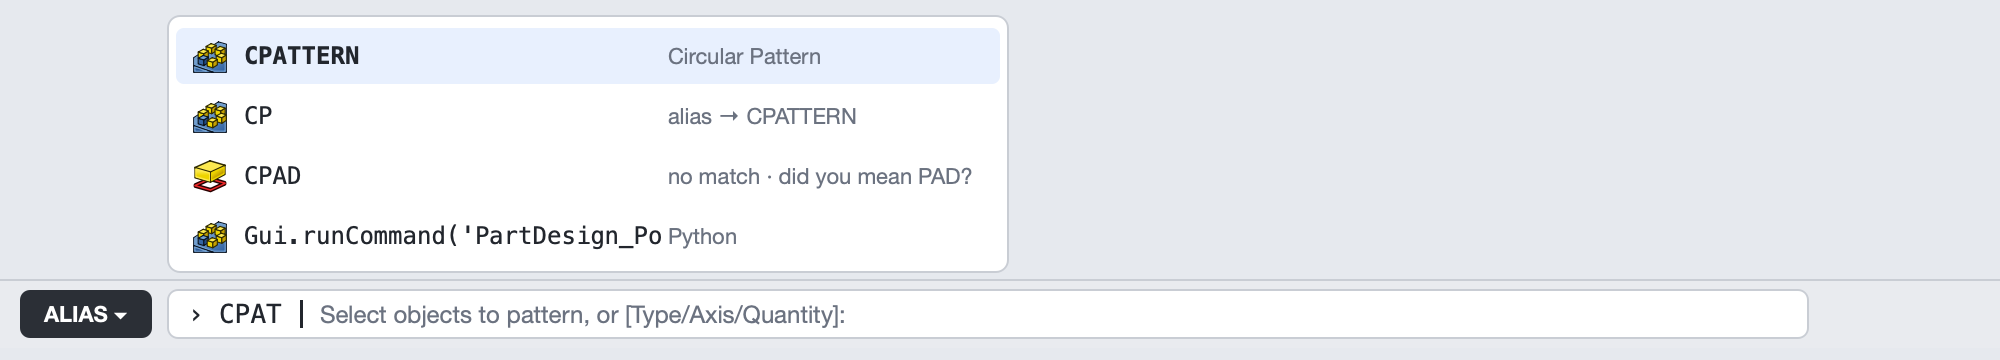
\includegraphics[width=\linewidth]{fig/cmdline.png}
\caption{Command line typing \code{CPAT} (working mock): ranked completions, the alias expansion, a ``did
you mean'' suggestion and the Python equivalent, with an AutoCAD-style \texttt{[Option/Option]} prompt.}
\end{figure}

\begin{figure}[ht]
\centering
\begin{tikzpicture}[>=Stealth,
  b/.style={draw=black!30,rounded corners=2pt,fill=white,minimum height=0.8cm,align=center,font=\small},
  m/.style={b,fill=bwblue!7,draw=bwblue!60}]
\node[b,minimum width=3cm] (in) {Command line\\\scriptsize\code{QLineEdit} + \code{CommandCompleter}};
\node[b,right=0.9cm of in,minimum width=2.4cm] (r) {Mode router\\\scriptsize prefix / mode chip};
\node[m,right=1cm of r,yshift=1.95cm,minimum width=4.2cm] (a) {Alias engine\\\scriptsize table $\to$ \code{Gui.runCommand} + prompts};
\node[m,right=1cm of r,yshift=0.65cm,minimum width=4.2cm] (p) {Python\\\scriptsize shared namespace with Python console};
\node[m,right=1cm of r,yshift=-0.65cm,minimum width=4.2cm] (c) {CadQuery / build123d\\\scriptsize exec $\to$ OCP shape $\to$ BREP};
\node[m,right=1cm of r,yshift=-1.95cm,minimum width=4.2cm] (o) {OpenSCAD\\\scriptsize \code{openscad} $\to$ CSG import};
\node[b,below=1.2cm of in,minimum width=3cm] (doc) {Document\\\scriptsize undo transaction};
\draw[->] (in) -- (r);
\foreach \x in {a,p,c,o} \draw[->] (r.east) -- (\x.west);
\draw[->] (a.east) -- ++(0.4,0) |- ($(doc.east)+(0,0.15)$);
\draw[->] (c.east) -- ++(0.6,0) |- ($(doc.east)+(0,-0.15)$);
\draw[->] (doc.north) -- node[left,font=\scriptsize]{prompt / result} (in.south);
\end{tikzpicture}
\caption{Command-line pipeline; each run is one undo transaction.}
\end{figure}

\paragraph{Design.} A bottom toolbar spanning the window, with focus key \code{:} or \code{Ctrl+`}. An
explicit mode chip (\code{ALIAS}/\code{PY}/\code{CQ}/\code{B3D}/\code{SCAD}) plus prefixes (\code{>>>},
\code{cq:}, \code{b3d:}, \code{scad:}), with alias mode as the default. Completion reuses FreeCAD's
\code{Gui::CommandCompleter}. Python runs in the console interpreter's namespace. OpenSCAD uses the
existing importer. No maintained add-on provides an AutoCAD-style line, and none bridges build123d into FreeCAD
(only the reverse, \code{ocp-freecad-cam}), so both are written here.

\paragraph{Theory: alias grammar and prompts.} Aliases live in a plain file in the spirit of AutoCAD's
\code{acad.pgp}. A line is parsed as
\begin{lstlisting}
line     := command ( WS arg )*
command  := ALIAS | COMMAND_NAME            ; case-insensitive
arg      := number unit? | option | ref
option   := IDENT                           ; matched against [A/B/C] prompt options
ref      := '@' object-label ( '.' subelement )?   ; e.g. @Flange.Face3
\end{lstlisting}
Missing arguments are asked for by a prompt state machine,
$\textsc{Select}\to\textsc{Option}^{*}\to\textsc{Value}^{*}\to\textsc{Commit}$. Viewport selection, a typed value or
Enter advances it, and Esc aborts the transaction.

\paragraph{Theory: ranking completions.} For query $q$ and candidate $c$,
\[
  \sigma(q,c) = 4\,[\,q \sqsubseteq_{\text{prefix}} c\,] + 2\,[\,q \sqsubseteq_{\text{initials}} c\,]
  + \frac{|q|}{\operatorname{span}(q,c)} + \lambda\log(1+f_c),
\]
where $\operatorname{span}$ is the shortest window of $c$ containing $q$ as a subsequence and $f_c$ is the
user's usage count. Unknown input gets the smallest Damerau--Levenshtein candidate (``did you mean PAD?'').

\paragraph{Theory: code-CAD bridge.} CadQuery and build123d wrap OCCT through OCP (pybind11), and FreeCAD
through \code{TopoShape}. Even when both load the same OCCT libraries, passing raw \code{TopoDS\_Shape}
pointers would couple two binding ABIs. The bridge therefore serialises through OCCT's BREP format:
$\texttt{OCP shape}\xrightarrow{\texttt{BRepTools::Write}}\text{BREP}\xrightarrow{\texttt{importBrepFromString}}\texttt{TopoShape}$.
Measured on the flange (15 faces, 10.9\,kB): 0.17\,ms to write and 0.12\,ms to read on the FreeCAD side,
with exact volume round-trip. The OCP-side write is still to be measured \verify.
\code{CodeFeature}s re-execute on recompute, so they start \emph{untrusted}, with recompute disabled until
the user approves them, the same trust model as FreeCAD macros.

\paragraph{Dependencies and the upstream-main decision.}
\begin{center}
\small
\begin{tabularx}{\linewidth}{@{}lllX@{}}
\toprule
Package (conda-forge) & Version & Needs & Fit with the current build (OCCT 7.8.1, Python 3.11)\\
\midrule
\code{ocp} & 7.8.1.2 & occt 7.8.1 \code{all\_h869bdd7\_203} & Same OCCT build hash as \file{pixi.lock} (osx-arm64)\\
\code{build123d} & 0.9.1 & ocp $\ge$7.8,$<$7.9 & OK\\
\code{cadquery} & 2.7.0 & ocp $\ge$7.8.1,$<$7.9 & OK, pin \code{<2.8}\\
\code{cadquery} & 2.8.0 & ocp 7.9.3.1 & Conflicts with OCCT 7.8\\
\code{openscad} & --- & --- & Not on conda-forge; separate binary\\
\bottomrule
\end{tabularx}
\end{center}
Tracking upstream main (\eref{FND-03}) means FreeCAD's OCCT will move to 7.9 or later. The OCP pin must then
move with it: CadQuery 2.8 already pairs with OCP 7.9.3. The pin is re-solved whenever the nightly
rebase changes \code{occt} in \file{pixi.toml}, and the command line's code-CAD modes are disabled with a
message, never broken, if no matching OCP exists yet.
